% !TeX encoding = UTF-8
% !TeX spellcheck = pt_BR

%%% PREAMBLE - Do not touch %%%%%%%%%%%%%%%%%%%%%%%%%%%%%%%%%%%%%%%%%%%%%%%%%%%%%%
\documentclass[10pt,twocolumn,letterpaper]{article}
\usepackage[utf8]{inputenc}	
\usepackage[portuges,brazil,english]{babel}
\usepackage{model}
\usepackage{times}
\usepackage{epsfig}
\usepackage{graphicx}
\usepackage{amsmath}
\usepackage{amssymb}
\usepackage{color}
\usepackage[pagebackref=true,breaklinks=true,letterpaper=true,colorlinks,bookmarks=false]{hyperref}
%  ABACO -- Conjunto de macros para desenhar o 'abaco
%  Desenho original de Hans Liesenberg
%  Macros de Tomasz Kowaltowski
%  DCC -- IMECC -- UNICAMP
%  Mar,co de 1988  --  Vers~ao 1.0
% Ajustado para LaTeX da SUN -- Mar,co de 1991
% ---------------------------------------------------------
%  Chamada:   \ABACO{d1}{d2}{d3}{d4}{esc}
%             com:  di's -- os quatro d'igitos;
%                   esc  -- fator de escala
% ---------------------------------------------------------
%  DEFINI,C~OES AUXILIARES
% ---------------------------------------------------------
%  Forma o d'igito pequeno (0 ou 1)

\newcommand{\ABACODP}[1]{%
%
\thicklines
%    
\begin{picture}(8,0)
    \ifcase#1{   %  caso 0
       \put(0,0)    {\line(1,0){4}}
       \multiput(5,0)(2,0){2}{\oval(2,4)}}
    \or{         %  caso 1
       \put(2,0)    {\line(1,0){4}}
       \multiput(1,0)(6,0){2}{\oval(2,4)}}
    \fi
\end{picture}
    } % \ABACODP

% Forma o d'igito grande (0 a 4)

\newcommand{\ABACODG}[1]{%
%
\thicklines
%    
\begin{picture}(14,0)
    \ifcase#1{   % caso 0
       \multiput(1,0)(2,0){5}{\oval(2,4)}}
       \put(10,0)   {\line(1,0){4}}
    \or{         % caso 1
       \multiput(1,0)(2,0){4}{\oval(2,4)}}
       \put(8,0)   {\line(1,0){4}}
       \put(13,0)   {\oval(2,4)}
    \or{         % caso 2
       \multiput(1,0)(2,0){3}{\oval(2,4)}
       \put(6,0)   {\line(1,0){4}}
       \multiput(11,0)(2,0){2}{\oval(2,4)}}
    \or{         % caso 3
       \multiput(1,0)(2,0){2}{\oval(2,4)}
       \put(4,0)   {\line(1,0){4}}
       \multiput(9,0)(2,0){3}{\oval(2,4)}}
    \or{         % caso 4
       \put(1,0)  {\oval(2,4)}}
       \put(2,0)   {\line(1,0){4}}
       \multiput(7,0)(2,0){4}{\oval(2,4)}
    \fi
\end{picture}
    } % \ABACODG
       
% Forma um d'igito (0 a 9)

\newcommand{\ABACOD}[1]{%
%
    \ifnum#1>9
       \errmessage{#1: Argumento invalido para ABACO}
    \fi
    \ifnum#1<0
       \errmessage{#1: Argumento invalido para ABACO}
    \fi
%
\begin{picture}(24,0)
%    
    \ifnum#1<5
       \put(16,0) {\ABACODP{0}}
    \else   
       \put(16,0) {\ABACODP{1}}
    \fi
%    
    \ifnum#1<5
       \put(0,0)  {\ABACODG{#1}}
    \else
       \ifcase#1\or \or \or \or
          \or  \put(0,0)  {\ABACODG{0}}
          \or  \put(0,0)  {\ABACODG{1}}
          \or  \put(0,0)  {\ABACODG{2}}
          \or  \put(0,0)  {\ABACODG{3}}
          \or  \put(0,0)  {\ABACODG{4}}
       \fi
    \fi   
\end{picture}
    } % \ABACOD
    
% -------------------------------------------------

%  DEFINI,C~AO PRINCIPAL
    
\newcommand{\ABACO}[5]{%
    \setlength{\unitlength}{#5mm}
%
    \thinlines
%   
\begin{picture}(28,25)
%   
% moldura
%
% externa
%
        \put(0,0)            {\line(0,1){25}}
        \put(0,0)            {\line(1,0){28}}
        \put(28,0)           {\line(0,1){25}}
        \put(0,25)           {\line(1,0){28}}
% interna
        \put(2,2)            {\line(0,1){21}}
        \put(26,2)           {\line(0,1){21}}
        \put(16,2)           {\line(0,1){21}}
        \put(18,2)           {\line(0,1){21}}
        \put(2,2)            {\line(1,0){14}}
%        \put(16,2)           {\line(1,-1){1}}
%        \put(17,1)           {\line(1,1){1}}
        \put(18,2)           {\line(1,0){8}}
        \put(2,23)           {\line(1,0){14}}
%        \put(16,23)          {\line(1,1){1}}
%       \put(17,24)          {\line(1,-1){1}}
        \put(18,23)          {\line(1,0){8}}
%        \put(0,0)            {\line(1,1){2}}
%        \put(0,25)           {\line(1,-1){2}}
%        \put(28,0)           {\line(-1,1){2}}
%        \put(28,25)          {\line(-1,-1){2}}
%
%   
% d'igitos
%
%   
       \put(2,20)  {\ABACOD{#1}}
       \put(2,15)  {\ABACOD{#2}}
       \put(2,10)  {\ABACOD{#3}}
       \put(2,5)   {\ABACOD{#4}}
%      
\end{picture}
    } % \ABACO
    


\cvprfinalcopy % *** Uncomment this line for the final submission
\def\httilde{\mbox{\tt\raisebox{-.5ex}{\symbol{126}}}}
\ifcvprfinal\pagestyle{empty}\fi

\newcommand{\TODO}[1]{TODO: #1}
\newcommand{\CITEONE}[2]{\mbox{#1 \cite{#2}}}
\newcommand{\CITETWO}[3]{\mbox{#1 and #2 \cite{#3}}}
\newcommand{\CITEN}[2]{\mbox{#1 et al. \cite{#2}}}

%%% Report beginning %%%%%%%%%%%%%%%%%%%%%%%%%%%%%%%%%%%%%%%%%%%%%%%%%%%%%%%%%%%%%%
\begin{document}

%%% Title and authors %%%%%%%%%%%%%%%%%%%%%%%%%%%%%%%%%%%%%%%%%%%%%%%%%%%%%%%%%%%%
\title{Usando regressão linear para prever a popularidade de notícias online}
\author{Mateus Coelho \thanks{\textbf{Contact}: \tt\small{mateus$\_$coelho@live.com}}}

%%% Abstract %%%%%%%%%%%%%%%%%%%%%%%%%%%%%%%%%%%%%%%%%%%%%%%%%%%%%%%%%%%%%%%%%%%%%
\maketitle

\begin{abstract}

Com a popularização da Internet e de redes sociais, meios de comunicação como jornais e revistas têm adquirido importância considerável devido à rápida divulgação de notícias. Assim, saber se uma notícia publicada na Web será popular ou não tornou-se um tópico quente da área de Machine Learning. Nesse projeto, utilizando um \textit{dataset} grande e de features diversificadas, esse problema foi abordado de maneira simples testando diversos modelos de regressão linear para estimar a quantidade de compartilhamentos de uma notícia. Após várias tentativas de modelos que forneciam medidas de erro absoluto médio entre 3000 e 3300, o melhor resultado foi obtido removendo notícias com mais de 20000 compartilhamentos do conjunto de treino e usando-o em um modelo de regressão linear simples com regularização. O erro absoluto médio foi de 2642 compartilhamentos, o qual não é satisfatório pois não é possível prever nada com segurança, já que 94$\%$ das notícias do conjunto de teste tem até 10000 mil compartilhamentos.

\end{abstract}

%%% Introduction %%%%%%%%%%%%%%%%%%%%%%%%%%%%%%%%%%%%%%%%%%%%%%%%%%%%%%%%%%%%%%%%%
\section{Introdução}

A previsão de popularidade de uma notícia publicada na Internet é um tópico quente na área de machine learning tendo em vista que vários trabalhos já foram publicados abordando técnicas diferentes e \textit{datasets} de diferentes meios de comunicação. Em geral, há duas maneiras de prever a popularidade: usando \textit{features} conhecidas somente após a publicação ou usando features pré-definidas. O primeiro modo é mais fácil e, geralmente, fornece resultados melhores do que o segundo modo. Existe também uma divisão na forma como a popularidade é estimada, já que alguns trabalhos estimam a quantidade de compartilhamentos que uma notícia terá e outros apenas classificam ela como popular ou impopular.

Usando o método de prever a popularidade com \textit{features} pré-definidas, alguns autores já conseguiram resultados interessantes. \CITEN{Petrovic}{sp} com um \textit{dataset} de 21 milhões de tweets tentou prever a quantidade de retweets usando \textit{features} relacionadas ao texto do tweet e a dados do autor. Fazendo uma classificação binária entre tweet e retweet, um F-1 \textit{score} de 47\%. \CITEN{Bandari}{rb}, com um \textit{dataset} correspondente a uma semana de notícias retiradas do Feedzilla, se propôs a classifica-las em 4 classes de popularidade tendo como valor de referência o número de tweets que mencionam um artigo. Fazendo uso de um conjunto diversicado de \textit{features} os melhores resultados foram de 77\% a 84\% de acurácia com os métodos Bayes e Bagging, respectivamente.
Por último, \CITEN{Fernandes}{kf}, que utilizou o mesmo \textit{dataset} que esse projeto, testou cinco modelos modernos para prever a quantidade de compartilhamento de notícias. Obteve o melhor resultado com o método \textit{Random Forests} e teve um \textit{discrimination power} de 73\%.

Tendo em vista estes bons resultados usando métodos que refletem o estado da arte em \textit{machine learning}, esse projeto analisou se é possível com métodos simples prever a popularidade de uma notícia. Para tanto, foi utilizado o clássico modelo de regressão linear com dois métodos de resolução, que foram \textit{gradient descent} e \textit{normal equations}. Além disso, um \textit{dataset} com 39000 notícias do popular site Mashable retiradas em 2015 também foi utilizado para treinar e testar os modelos propostos.

%%% Add section %%%%%%%%%%%%%%%%%%%%%%%%%%%%%%%%%%%%%%%%%%%%%%%%%%%%%%%%%%%%%%%%%%
\section{Soluções Propostas}

\subsection{Conjunto de dados}

O conjunto de dados utilizado neste \textit{paper}, foi criado e disponibilizado por \CITEN{Fernandes}{kf}, apresenta 39797 notícias retiradas do popular site de notícias Mashable no idioma inglês. O \textit{dataset} como foi dispobilizado tem 61 \textit{features}, sendo 58 atributos preditivos, 2 não preditivos (URL e tempo entre mineração e publicação) e 1 objetivo, que é a quantidade de compartilhamentos. Os dados foram coletados entre janeiro de 2013 e janeiro de 2015 e os artigos que não poderiam ser tratados automaticamente foram removidos, assim como os artigos mais recentes (até quatro semanas). Os atributos do conjunto de dados podem ser dividos em 6 categorias: palavras, \textit{links}, mídia digital, data, palavras-chave e processamento de linguagem natural. O valor de todos os atributos são booleanos, números ([0,$\infty$]) ou razões ([0-1]). Mais informações sobre o \textit{dataset} podem ser obtidas na sua página no repositório UCI Machine Learning.

Antes de começar a testar os modelos foram efetuadas pequenas alterações no \textit{dataset}. Os atributos não preditivos foram removidas, o atributo \textit{É fim de semana?} foi removido pois tem informação repetida e um atributo com todos os valores iguais a 1 foi adicionado pois correspondente à \textit{feature} que multiplica o coeficiente linear da função utilizada para predizer o valor de compartilhamentos. Além disso, os 7 atributos que indicam o dia semana em que a notícia foi publicada foram substituídas por 3 três atributos binários que juntos correspondem ao número do dia em base binária, por exemplo 010 corresponde a terça-feira.

\subsection{Modelos}

Primeiramente foi testado o modelo de regressão linear básico correspondente à equação \ref{eq:reglin} com todas as \textit{features} disponíveis. Foram testados também modelos lineares com termos quadrados e cúbicos dos atributos. Em uma tentativa mais extrema de tratar os atributos discretos do \textit{dataset}, a equação \ref{eq:reglin} foi aplicada com todas os atributos menos os discretos.

\begin{equation}
	h_{\theta} = \theta_1 + x_1 \theta_2 + x_2 \theta_3 + \dots +  x_n \theta_n
	\label{eq:reglin}
\end{equation}

A partir da aplicação do método de \textit{Random Forests} efetuado por \CITEN{Fernandes}{kf} no mesmo \textit{dataset}, foram obtidas as 10 \textit{features} mais importantes, que são:

\begin{enumerate}
	\item Palavra-chave média (média de compartilhamentos).
	\item Palavra-chave média (máximo de compartilhamentos).
	\item Proximidade do terceiro tópico mais relevante do LDA.
	\item Categoria do artigo 
	\item Quantidade mínima de compartilhamento de links do Mashable
	\item Melhor palavra-chave (média de compartilhamentos).
	\item Quantidade média de compartilhamento de links do Mashable
	\item Proximidade do segundo tópico mais relevante do LDA.
	\item Pior palavra-chave (média de compartilhamentos).
	\item Proximidade do quinto tópico mais relevante do LDA.
\end{enumerate}

Assim, o modelo da equação \ref{eq:reglin} também foi aplicado para apenas esses 10 atributos.

Vale ressaltar que a regularização também foi utilizada em todos os modelos mesmo sem \textit{overfitting}.

%%% Add section %%%%%%%%%%%%%%%%%%%%%%%%%%%%%%%%%%%%%%%%%%%%%%%%%%%%%%%%%%%%%%%%%%
\section{Experimentos e discussão}

Para realizar os testes foram desenvolvidos os algoritmos \textit{gradient descent} e \textit{normal equations} em Python com bibliotecas auxiliares como \textit{pandas} e \textit{numpy}, sem entretanto usar bibliotecas que já tinham soluções prontas.

A respeito desse métodos de minimizar a \textit{coast function} ($J(\theta)$) percebeu-se uma clara vantagem do segundo especialmente para casos em que a quantidade de \textit{features} a serem analisadas era pequena (menor que 200). Além disso, foram obtidos melhores resultados usando \textit{normal equations} porque para ter um valor parecido usando \textit{gradient descent} era necessário fazer muitas iterações, o que demoraria muito para ser processado. Note que as condições de parada do método iterativo foram: diferença entre coast functions menor que 10 ou número máximo de iterações igual a 50000. Portanto, os resultados expostos neste \textit{paper} são os conseguidos pelo \textit{normal equations} apesar de ambos serem testados.

Ao aplicar o gradient descent foram plotados gráficos de coast function vs. número de iterações, mas todos têm obviamente o mesmo formato, mudando apenas o valor da coast function. Um exemplo desse gráfico pode ser visto na figura \ref{fig:complex}, que corresponde ao primeiro e mais básico modelo testado sem regularização. Para aumentar a rapidez da convergência foi empregado também a normalização da média em todas os atributos que não tinham valores entre -1 e 1.

\begin{figure}
\begin{center}
	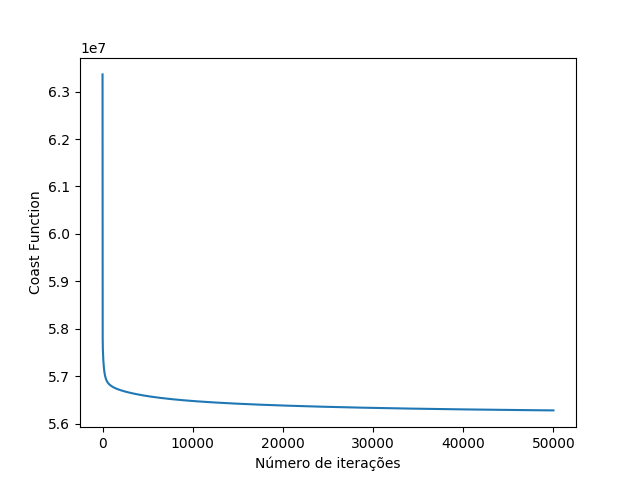
\includegraphics[width=0.99\columnwidth]{pics/curva.png}
	\caption{Convergência do gradient descent.}
	\label{fig:complex}   
\end{center} 
\end{figure} 

Com relação ao uso do dataset para treinar e testar os modelos, foi respeitada uma repartição de 80\% para o conjunto de treino e 20\% para o conjunto de treino. Ademais, nos casos em que regularização foi aplicado, o método de cross-validation foi empregado para encontrar o valor ideal do parâmetro $\lambda$ da regularização. A proporção foi de 80\% do conjunto de treino para efetivamente treinar e 20\% do conjunto de treino para encontrar o parâmetro.

De maneira geral os resultados foram ruins já que os valores do erro médio absoluta (MAE) foram altos. A tabela \ref{tab:result} mostra resumidamente os erros para os modelos especificados na seção anterior. Já que os valores de compartilhamentos no conjunto de teste são quase todos abaixo de 10000, pode-se concluir que a função preditora tem uma precisão muito baixa. 

O gráfico da função preditora e dos valores reais de compartilhamento para o modelo básico pode ser visualizado na figura \ref{fig:funcao}, na qual o eixo x indica o número do caso do conjunto de teste. Com ele, pode-se perceber que existem alguns casos em que o valor de compartilhamento real é muito alto e a função não acompanha. Além disso, é patente que a maioria dos casos do \textit{dataset} tem valores baixos do atributo objetivo.

A solução, então, que resultou no melhor erro foi remover alguns casos do conjunto de treino que tinham valores de compartilhamentos altos. Assim o modelo ficaria mais ajustado aos casos que são maioria no conjunto de teste. Esse processo foi realizado de forma gradual ao longo de três iterações e testando o modelo da equação \ref{eq:reglin} para verificar se o erro seria menor. Os erros dos testes nessas três iterações podem ser visualizados na tabela \ref{tab:resultbom}.

A remoção foi feita plotando o gráfico de cada \textit{feature} pela quantidade de compartilhamentos e retirando pontos (casos) que estavam distantes da maior concentração de pontos. Foram removidos pouco mais de 1000 casos que tinham a maior quantidade de compartilhamentos do conjunto de treino.

\begin{table}[]
\centering
\caption{Resultados após remoção de casos do conjunto de treino}
\label{tab:resultbom}
\begin{tabular}{ll}
Modelo & MAE \\
Eq \ref{eq:reglin} com regularização e remoção de 33 casos & 3110 \\
Eq \ref{eq:reglin} com regularização e remoção de 226 casos & 3082 \\
Eq \ref{eq:reglin} com regularização e remoção de 1235 casos & 2642
\end{tabular}
\end{table}

\begin{figure}
\begin{center}
	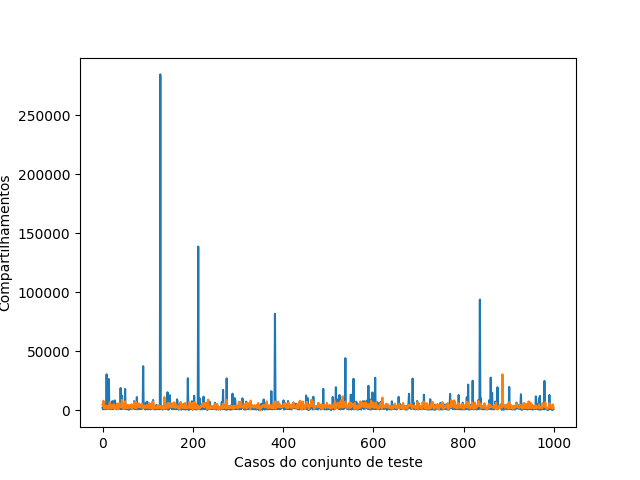
\includegraphics[width=0.99\columnwidth]{pics/funcao.png}
	\caption{Comparação entre valores dados pelo modelo e os valores reais de compartilhamentos.}
	\label{fig:funcao}   
\end{center} 
\end{figure}

\begin{table}[]
\centering
\label{tab:result}
\caption{Erros dos diversos modelos testados}
\begin{tabular}{ll}
Modelo & MAE \\
Eq \ref{eq:reglin} & 3181 \\
Eq \ref{eq:reglin} com regularização & 3210 \\
Eq \ref{eq:reglin} com quadrados & 3181 \\
Eq \ref{eq:reglin} com quadrados e regularização & 3152 \\
Eq \ref{eq:reglin} com cubos & 3181 \\
Eq \ref{eq:reglin} com cubos e regularização & 3146 \\
Eq \ref{eq:reglin} sem atributos discretos & 3186 \\
Eq \ref{eq:reglin} sem atributos discretos com reg. & 3186 \\
Eq \ref{eq:reglin} com top 10 atributos & 3184 \\
Eq \ref{eq:reglin} com top 10 atributos e reg. & 3184
\end{tabular}
\end{table}

%%% Add section %%%%%%%%%%%%%%%%%%%%%%%%%%%%%%%%%%%%%%%%%%%%%%%%%%%%%%%%%%%%%%%%%%
\section{Conclusões e direções futuras}

O objetivo do projeto é verificar se é possível obter uma boa estimativa da quantidade de compartilhamentos que uma notícia terá usando modelos simples de regressão linear. Os resultados obtidos mostram que não é possível pois o erro é muito grande comparado com os valores de compartilhamentos reais. O melhor resultado teve um MAE de 2642, mas ainda não é satisfatório pois 94$\%$ das notícias do conjunto de teste tem até 10000 mil compartilhamentos.

Algumas opções que poderiam ser testadas em uma eventual continuação deste projeto são testar modelos mais complexos de regressão com multiplicação de \textit{features} ou eleva-las a graus maiores, como 25 ou 50. Além disso pode-se verificar se remover mais casos do conjunto de treino ajuda a função preditora a ficar mais ajustada e reduzir o erro. 

%%% References %%%%%%%%%%%%%%%%%%%%%%%%%%%%%%%%%%%%%%%%%%%%%%%%%%%%%%%%%%%%%%%%%%%
{\small
\bibliographystyle{unsrt}
\bibliography{refs}
}


\end{document}